
%
%  void-input - easy report template for included file
%  EDIT THE LINE ABOVE FOR DOCUMENTATION OF THIS FILE, then delete this line! 
%         

%

% ============================================================
% --- texstudio magic comment: 
% !TEX encoding = UTF-8
% !TeX program = pdflatex
%% !TeX program = xelatex
% !TeX root = "cognome-tesina.tex"
% %  !TeX spellcheck = en_US
% !TeX spellcheck = it_IT


% ====================================================================


\chapter{Task 1}
The first tsk was very simple and did not include anything new compared to what has already been done in previous experiences. There are therefore no particular things to say.

\chapter{Task 2}
The second task, like the first, was not as complex. It simply required im- plementing a callback function on click. The ”hardest” part was figuring out how to use pointers. But equally dedicating a few extra minutes there was no problem.


\chapter{Task 3}
For this task it was sufficient to slightly modify the code of the previous task also taking the neighboring values and finally making the average. Again I arrived at the solution without too much trouble.


\chapter{Task 4}
This fourth task was slightly longer than the previous ones due to some very simple error occurred due to incorrect copy and paste (for example it gave me segmentation fault because by mistake copying and pasting one of the for loops necessary for iteration, I forgot to replace the variable with the new one). But apart from this simple typo, I haven’t had any problems or difficulties writing the code here either. In the images below you can see the results of the mask when you clicked on the ball with a THRESHOLD of 80. Obviously, being the color very similar to that of the football robot shirt, portions of the shirts are colored equally in the mask. On the left the Figure \ref{fig:4a} is the original one while on the right (Figure \ref{fig:4b}) we can see the generated mask.


\begin{figure}[h]
	\centering
	\begin{minipage}{0.45\textwidth}
		\centering
		
\includegraphics[width=\linewidth]{images/source/2}
		\caption{Original Image.}
		\label{fig:4a}
        \end{minipage}
        \hspace{0.05\textwidth}
        \begin{minipage}{0.45\textwidth}
        		\centering
		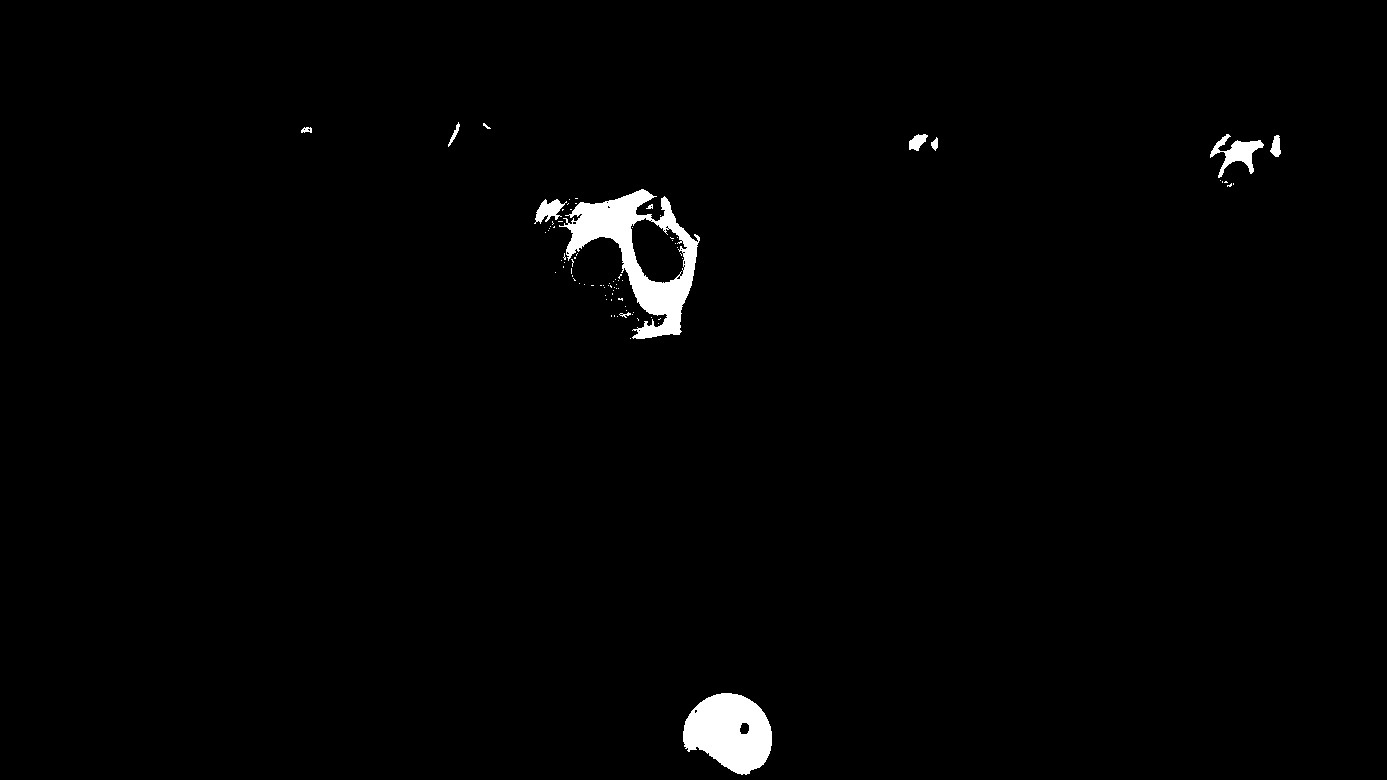
\includegraphics[width=\linewidth]{images/source/task4/1}
		\caption{Mask of the image based on the click on top of the ball.}
		\label{fig:4b}
        \end{minipage}
\end{figure}


\chapter{Task 5}
In this last task I made a simple modification to the fourth task to use the pixels of the original color coming from the image instead of the black ones and to signal the color pixels similar to the ones clicked instead of white I used the required value of (92, 37, 201).
In this case I used a THRESHOLD of 90 just to make further tests.
The Figure \ref{fig:5a} shows the original image. The Figure \ref{fig:5b} show the image after selecting some of the elements.

\begin{figure}[h]
	\centering
	\begin{minipage}{0.45\textwidth}
		\centering
		
\includegraphics[width=\linewidth]{images/source/2}
		\caption{Original Image.}
		\label{fig:5a}
        \end{minipage}
        \hspace{0.05\textwidth}
        \begin{minipage}{0.45\textwidth}
        		\centering
		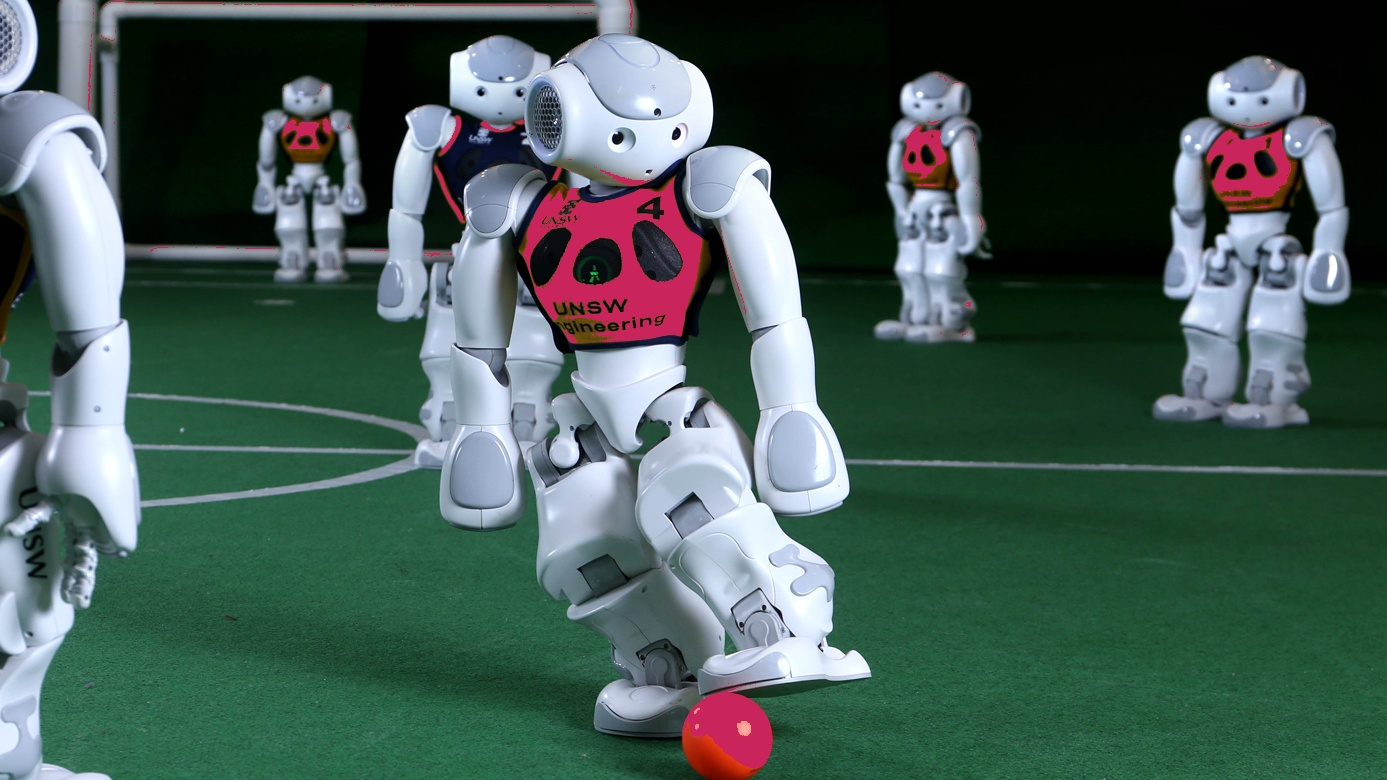
\includegraphics[width=\linewidth]{images/source/task5/1}
		\caption{Selection based on the click on the T-shirt.}
		\label{fig:5b}
        \end{minipage}
\end{figure}




% ====================================================================

% ====================================================================
% memo available commands
% ====================================================================
% easyrep: summary of provided macros
%
% \Title{text}     defines the document title 
% \Subtitle{text}  defines the subtitle
% \Author{text}    defines the author string
% \Date{text}      defines a date string
% \printCover      print a cover page using above information
%
% --- text styles
% \tDef{text}      definition (generic) 
% \tDefObj{text}   definition (the ter being defined)
% \tDefTxt{text}   definition (the statement defining the term) 
% \tRemark{text}   remarked text
% \tREMARK{text}   highly remarked text 
% \tLoud{text}     shouted text! 
% \tCode{text}     inline code text
% \tLatin{text}    latin text
% \tForeign{text}  foreign language text 
% \tExample{text}  example 
% \tStandard{text} a recommendation 
% \tQuote{text}    a quoted text 
% \tQuoteFig{text} a quoted text referring to a figure 
% \tConcept{text}  an important concept  
% \tBeginPar{text} highlighted text 
%                  at the beginning of a paragraph 
%
% ---environments
% \begin{quoteStandard} text... \end{quoteStandard}
%    print text to be quoted, e.g. sentences from 
%    a recommendation
%
% \begin{quoteRemark} text... \end{quoteRemark}
%    similar to quoteStandrd, but the text is more marked
%
%  
% --- typo accelerators
% \qmo             opening quotation mark (use \qmo{})
% \qmc             closing quotation mark (use \qmc{})
% \th  emphasises "th"
% \ie  slanted "i.e."
% \eg  slanted "e.g."
% \es  slanteg "ad es."
% \octave   "octave" in \tCode style
% \matlab   "matlab"
% \labview  "labVIEW"
% \latex    "LaTeX" (just the text!)
%
% --- math typo accelerators
% \v{math text}  underlines the math text (useful for vector) 
%
% --- debug commands
% \debugTextStyles        print a table showing text styles
% \debugPrintCharacters   print a table of characters
% \Vispa                  print some text (to fill)  
% \Vispas                 more filling text
% ====================================================================
